% !TEX encoding = UTF-8
% !TEX TS-program = pdflatex
% !TEX root = ../tesi.tex

%**************************************************************
\chapter{Dominio aziendale}
\label{cap:introduzione}
In questo capitolo viene descritta l’azienda ospitante in cui è stata
svolta l’attività.

%\emph{api}
%\noindent Esempio di utilizzo di un termine nel glossario \\


%\noindent Esempio di citazione in linea \\
%\cite{site:agile-manifesto}. \\

%\noindent Esempio di citazione nel pie' di pagina \\
%\footcite{http://www.zero12.it/} \\


\section{L'azienda ospitante}
\begin{figure}[!h] 
	\centering 
	
\includegraphics[width=0.5\columnwidth]{azienda} 
	\caption{Logo di Nextep: immagine tratta dal sito dell’azienda}
\end{figure}
Nextep è una società fondata nel 2000 da Marco De Toni e Mirco Soffia, con sede
attuale a Cittadella (PD).
Opera nel settore informatico e si occupa di servizi web, web marketing e di infrastrutture
per gestire le informazioni delle aziende, e più in generale ha come obiettivo
quello di migliorare l’efficacia delle strategie di comunicazione web, delle aziende,
dedicando particolare attenzione alla reputazione e all’identità digitale. 
\\

Nextep fa parte del gruppo Allos, insieme ad Allos Italia\footcite{https://www.allos.it/}, Allos Sud Africa\footcite{http://www.allos.co.za/}, Allos
USA\footcite{http://www.allosamerica.com/} e Zero12\footcite{http://www.zero12.it/}.
Allos si occupa di progetti e tecnologie per lo sviluppo del capitale umano, mentre
Zero12 si occupa dello sviluppo di soluzioni mobile e cloud based.
Il gruppo Allos è stato recentemente acquisito da EOH Holdings Ltd\footcite{http://www.eoh.co.za/}, una grande
società sudafricana.
\\

Nextep ha un organico di circa venti persone, tra dipendenti e collaboratori, con
varie competenze: grafici, sviluppatori, esperti di web marketing e tecnici. Sono presenti
tre gruppi principali di lavoro: quello di sviluppo, creativo e del supporto
tecnico.
In Nextep c’è un ambiente di lavoro giovane, dinamico ma allo stesso tempo professionale,
ed è incentivata la collaborazione e la condivisione di conoscenze e idee
tra le persone. Tutto questo favorisce sia la crescita individuale, dal punto di vista
professionale, che la crescita e l’amalgamazione dei vari gruppi di lavoro.

%**************************************************************\newpage
\section{Prodotti e servizi}
Nextep lavora per clienti di diversa tipologia e conformazione, dalla piccola impresa
privata alla multinazionale che si sta espandendo ulteriormente, e con questo offre
svariati prodotti e servizi in base alle esigenze e alle opportunità del mercato e proprie. 
\\

La maggior parte dei progetti riguarda la realizzazione di portali e siti web, ma vengono
sviluppati anche diversi altri prodotti, tra cui soluzioni e-commerce e applicazioni
mobile, sviluppo di progetti di virtualizzazione, e storage networking. Inoltre negli ultimi mesi l'azienda si sta dedicato molto anche ai prodotti di \emph{machine learning}, come i chatbot. \\

Nextep offre diversi tipi di servizi tra questi l'installazione e assistenza del portale di \emph{customer service} Zendesk. Guida le diverse società(piccole o grandi) verso la gestione dei proprio cliente in maniera semplice ed efficace. 
%**************************************************************

\section{Metodologia organizzativa utilizzate da Nextep}
Pur avendo lavorato al progetto autonomamente, e quindi non direttamente insieme
al personale, ho potuto constatare alcuni metodi utilizzati
dall’azienda. 
\\
 
Il team di Nextep segue una metodologia di sviluppo agile: il framework Scrum.
Scrum è un framework che ha lo scopo di affrontare complessi problemi adattivi
e collaborativi, per realizzare prodotti di alto valore in modo sia produttivo che creativo.
Questo approccio permette di essere flessibili di fronte a imprevisti e a cambiamenti
nei requisiti, molto frequenti all’interno di progetti innovativi e personalizzati che
l’azienda offre.
\\
\begin{figure}[!h] 
	\centering 
	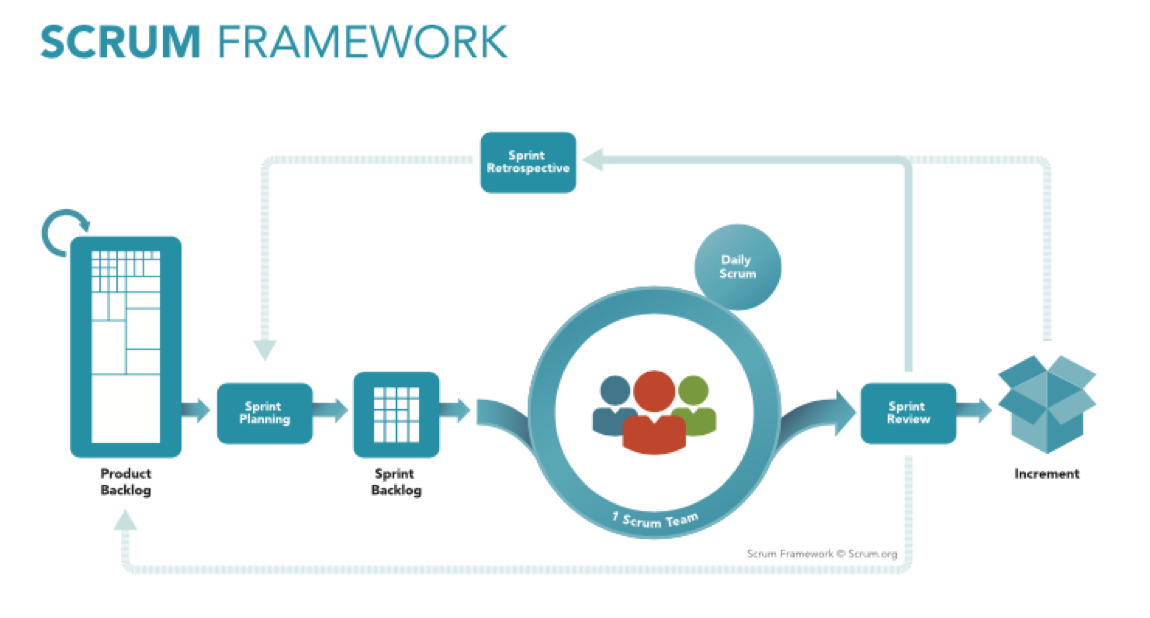
\includegraphics[width=0.8\columnwidth]{scrum} 
	\caption{Logo di Nextep: immagine tratta dal sito dell’azienda}
\end{figure}
\newpage
Secondo questa metologia il team è formato da: 
\begin{itemize}
	\item \textbf{Product owner:} responsabile della gestione dei product backlog e della
	volontà degli stakeholder;
	\item \textbf{Scrum master:} responsabile del team, si assicura che le regole di Scrum
	vengano applicate e che il team sia il più produttivo possibile;
	\item \textbf{Development team:} team con competenze tecniche, che lavora insieme per
	completare l’incremento di uno sprint.
\end{itemize}

Dove gli artefatti dello Scrum sono: 
\begin{itemize}
	\item \textbf{Product Backlog:} lista ordinata, in base alle priorità, di tutti i requisiti che
	il prodotto deve soddisfare;
	\item \textbf{Sprint Backlog:} lista dei compiti, presi dal Product Backlog, che il team di
	sviluppo deve completare nello sprint corrente;
	\item \textbf{Increment:} somma di tutti i requisiti del Product Backlog che sono stati
	completati.
\end{itemize}

Inoltre lo Scrum definisce diversi tipologie di riunioni, ogniuna con la durata diversa e con l'obbiettivo di organizzare il lavoro tra i membri del team. Nella azienda in questione, ogni giorno è previsto uno \emph{stand-up meeting} all’interno dei vari team di
lavoro, per allineare ogni componente sulla situazione corrente e su come procedere. 


\section{Principali strumenti utilizzati da Nextep}
Come cenato prima, l'azienda si occupa princiaplamente delle applicazione web. La realizzazione delle applicazione viene fatto utilizzando i CMS di PHP, come:
\begin{itemize}

	\item \textbf{Drupal:} una piattaforma software, flessibile e scalabile, per la creazione e pubblicazione
	di siti web, e per la condivisione di contenuti in più linguaggi su
	dispositivi diversi;
		\item \textbf{Wordpress:} un'altra piattaforma software, che consente la creazione e
	distribuzione di siti web facilmente gestibili ed aggiornabili in maniera dinamica.
\end{itemize}

Per quanto riguarda controllo del versionamento e CI/CD(\emph{continuous integration and delivery}) l 'azienda utlizzata Git e Gitlab (descritti in detaglio nel capitolo 3).
\\

Per quanto riguarda la gestione dei ticketing viene adoperato Jira, un software proprietario per l’issue tracking, bug tracking
e con funzioni di gestione del progetto.

